 \documentclass{article}
\usepackage{tikz}
\usetikzlibrary{angles, quotes}
\usepackage{amssymb}
\usepackage{pgfplots}
\pgfplotsset{width=10cm,compat=1.9}
\usepgfplotslibrary{statistics}
\usepackage[left=2.54cm,right=2.54cm,top=2.54cm,bottom=2.54cm]{geometry}
\usepackage{tasks} %Paquete necesario para la producción de items horizontales para algunos ejercicios de tarea empleando el comando /begin{multicols}}{#}.../end{multicols} para ayudarnos a reducir las páginas
\usepackage{pdflscape} %comando que permite cambiar a orientación horizontal las hojas%
\usepackage{soul} %Paquete para permitir la compilación de acentos usando el comando {\hl{}}}\\
\sethlcolor{yellow(munsell)} %comando para definir el color para el subrayado usando el comando \hl
\usepackage[utf8]{inputenc}
\usepackage[spanish]{babel}
\usepackage{icomma}
\usepackage{ragged2e}
\usepackage{siunitx}
\usepackage{url}
\usepackage[colorlinks=true, urlcolor=blue,  linkcolor=black, citecolor=green]{hyperref}
\usepackage{pdfpages}
\usepackage{blindtext} %Paquete que genera texto ficticio (dummy text) con el comando: \blindtext
\usepackage{cancel} %in the preamble gives you four different modes of striking through: \cancel{text to cancel} draws a diagonal line (slash) through its argument, \bcancel{text to cancel} uses the negative slope (a backslash), \xcancel{text to cancel} draws an X (actually \cancel plus \bcancel), \cancelto{〈value〉}{〈expression〉} draws a diagonal arrow through the 〈expression〉pointing to the 〈value〉 (math-mode only)
\usepackage{csquotes}
\usepackage{afterpage}
\usepackage{parskip} 
\usepackage{float}
\usepackage{enumitem}
\usepackage{multicol}%Paquete que permite la creación aislada de columnas de texto. De esta forma se reduce la cantidad de páginas en nuestro documento
\usepackage{lipsum} %Paquete que genera texto de relleno al igual que \usepackage{blindtext}, se usa con el comando \lipsum[#-#] los #(hashtags) delimitan el número de páginas que deseamos ocupar del paquete lipsum para usarlos como relleno. 

% Definir el comando personalizado para la nota
\newcommand{\mynote}[1]{%
\begin{tikzpicture}[baseline=-0.75ex]
\node[draw, circle, fill=Apple Green!60, inner sep=2pt] (note) {\textbf{Nota:}};
\end{tikzpicture}%
\ \textit{#1}%
}

\newenvironment{Figura}
{\par\medskip\noindent\minipage{\linewidth}}
{\endminipage\par\medskip}
\usepackage{caption}
\usepackage[
backend=biber,
sorting=none,
url=true
]{biblatex} %bibliografía
\addbibresource{biblio.bib}
% Establecer el espacio entre las entradas de la bibliografía
\setlength{\bibitemsep}{1\baselineskip} % Puedes ajustar el valor según tus preferencias
\usepackage{amsmath,amsthm,amssymb,amsfonts}
\usepackage{pifont} %Permite la compilación del comando \xmark: es el símbolo de la tachita
\usepackage{mathtools} %permite la compilación de símbolos para matrices
\usepackage{empheq} %Paquete que se relaciona con \usepackage[most]{tcolorbox} para la creación de cuadros/cajas de colores para delimitar los resultados matemáticos o líneas de texto usando la línea de comando: \begin{empheq}[box={\mymath[colback=orange(webcolor)!70,drop lifted shadow]}]{equation*} \end{empheq}
\usepackage[most]{tcolorbox} %Paquete que se relaciona con \usepackage{empheq} para la creación de cuadros/cajas de colores para delimitar los resultados matemáticos o líneas de texto
\renewcommand{\qedsymbol}{$\blacksquare$}
\usetikzlibrary{positioning,decorations.pathreplacing} %Paquete que permite la compilación de llaves para cuadros sinópticos (brace diagram) 
\usepackage{schemata} %The schemata package is designed just for these brace diagrams
\usepackage{booktabs}

\newcommand\AB[2]{\schema{\schemabox{#1}}{\schemabox{#2}}} %comando o paquete necesario para crear cuadros sinópticos

\newtcbox{\mymath}[1][]{%
nobeforeafter, math upper, tcbox raise base,
enhanced, colframe=blue!30!black,
colback=blue!30, boxrule=1pt,
#1} %Comando importante para encasillar los resultados matemáticos en cajas de diferentes colores, se relaciona con los paquetes \usepackage{empheq} y \usepackage[most]{tcolorbox} 

\newenvironment{sysmatrix}[1]
{\left(\begin{array}{@{}#1@{}}}
{\end{array}\right)}
\newcommand{\ro}[1]{%
\xrightarrow{\mathmakebox[\rowidth]{#1}}%
}
\newlength{\rowidth}% row operation width
\AtBeginDocument{\setlength{\rowidth}{3em}}  %Comando importante para laproducción de lineas de operaciones entre matrices, método de Gauss o Gauss Jordan se relaciona con \newenvironment{sysmatrix}

%formato para cambiar el horario a español
\usepackage[spanish]{datetime2}
\DTMsetdatestyle{spanish}

\renewcommand{\today}{\DTMdisplaydate{\the\year}{\the\month}{\the\day }{-1}}
%%%%%%%%%%%%%%%%%%%%%%%%%%%%%%%%%%%%%%%%%

\usepackage{datetime}
\newcommand{\mycurrenttime}{\xxivtime}

%%%%%%%%%%%%%%%%%%%%%%%%%%%%%%%%%%%%%%%%%%%%%%%%%%%%%%%%%%%%%%%%%%%%%%%%%%%%%%%%%%%%%%%%%%%%%%%%%%%%%%%%%%%%%%%%%%%%%%%%%%%%%%%%%%%%%%%%%%%%%%%%%


%%%%%%%%%%%%%Caja de color para el título%%%%%%%%%%%%%%%%%%%%%%%%%%%%%%%%%%%%%%%%%%%%%%%%%%%%%%

\definecolor{myframecolor}{RGB}{1, 45, 75} % Prussian Blue
\definecolor{myboxcolor}{RGB}{0, 107, 92} % Apple Green

\newtcolorbox{mybox}{
enhanced,
colback=myboxcolor!7, % Color de fondo del cuadro
colframe=myframecolor, % Color del marco del cuadro
arc=0pt,
boxrule=1pt,
borderline west={2mm}{-10mm}{myframecolor}, % Borde en el lado izquierdo
sharp corners=southwest,
width=\linewidth,
before=\par\vspace{\bigskipamount}, % Espacio antes del cuadro
after=\par\vspace{\bigskipamount} % Espacio después del cuadro
}


\newcommand{\euler}{e} %Comando para producir letra e de euler
\newenvironment{remark}{\par\vfill\footnotesize % Vertical white space above the remark and smaller font size
\begin{list}{}{
	\leftmargin=80pt % Indentation on the left
	\rightmargin=60pt}\item\ignorespaces % Indentation on the right
\makebox[-2.5pt]{\begin{tikzpicture}[overlay]
		\node[draw=Horizon!60,line width=2.5pt,circle,fill=Horizon!25,font=\sffamily\bfseries,inner sep=4pt,outer sep=0pt] at (-19pt,5pt){\textcolor{Horizon}{Nota}};\end{tikzpicture}} % Blue Nota in a circle
\advance\baselineskip -1pt}{\end{list}\vskip5pt} % Tighter line spacing and white space after remark
\usepackage{graphicx}

\usepackage{titling}

\input{colores.tex}

%%Producir signos de cita textual``Asignatura''

\newcommand{\xmark}{\ding{55}} %%%comando que genera la tachita

\newenvironment{MyColorPar}[1]{%
\leavevmode\color{#1}\ignorespaces%
}{%
}%

%%%%%%%%%%%%%%%%%%% Título de la tarea, Nombre de alumno

\title{Clase \#29 - Electrodinámica}
\author{\emph{Julio Alfredo Ballinas García} $\boldsymbol{\mid}$ 202107583}
\date{\today}

%%%%%%%%%%%%%%%%%%% Datos de la Materia

\usepackage{fancyhdr}
\fancypagestyle{plain}{%  the preset of fancyhdr 
\fancyhf{} % clear all header and footer fields
\fancyfoot[R]{
\includegraphics[width=2cm]{LogoFCFMBUAP (1).png}}
\fancyfoot[L]{{\bfseries{\thedate{}}} a las {\bfseries{\mycurrenttime{}}} horas{} (GMT-6, H. Puebla de Zaragoza, Pue)}
\fancyhead[L]{Electrodinámica}
\fancyhead[R]{\theauthor}
}
\makeatletter
\def\@maketitle{%
\newpage
\null
\vskip 1em%
\begin{center}%
\let \footnote \thanks
{\LARGE \@title \par}%
\vskip 1em%
%{\large \@date}%
\end{center}%
\par
\vskip 1em}
\makeatother

\usepackage{lipsum}  
\usepackage{cmbright}


%%%%%%%%%%%%%%%%%%%%%%%%%%%%%%%%%%%%%%%%%%%%%%%%%%%%%%%%%%%%%%%%%%%%%%%%%%%%%%%%%%%%%%%%%%%%%%%%%%%%%%%%%%%%%%%%%%%%%%%%%%%%%%%%%%%%%%%%%%%%%%%%%%%%%%%%%%%%%%%%%%%%%%%%%%%%%%%%%%%%%%%%%%%%%%%%%%%%%%

\begin{document}



\maketitle


%%%%%%%%%%%%%%%%%%% Datos del profesor, campus y aula

\begin{mybox}
\noindent\begin{tabular}{@{}ll}
	{\bfseries{Profesor}} & Dr. Iván Fuentecilla Cárcamo\\
	\textcolor{prussianblue}{\bfseries{Campus}} / \textcolor{trueblue}{\bfseries{Facultad}}  & \textcolor{prussianblue}{\bfseries{C.U. BUAP}} /  \textcolor{trueblue}{\bfseries{FCFM}} \\
	\textcolor{prussianblue}{\bfseries{Edificio}} /  \textcolor{trueblue}{\bfseries{Salón}}    & 	\textcolor{prussianblue}{\bfseries{EMA4}} /  \textcolor{trueblue}{\bfseries{409}}   
\end{tabular} 
\end{mybox} \vspace{1cm}




	





\begin{MyColorPar}{orange(colorwheel)}

\end{MyColorPar}


\tableofcontents \newpage

\begin{center}
\begin{tikzpicture}
	% Dibuja círculos rellenos en diferentes colores
	\fill[bittersweet] (0,0) circle (0.17cm);
	\fill[Apple Green] (0.6,0) circle (0.17cm);
	\fill[trueblue] (1.2,0) circle (0.17cm);
	\fill[Aguamarina] (1.8,0) circle (0.17cm);
	\fill[Sun] (2.4,0) circle (0.17cm);
	\fill[orange(colorwheel)] (3.0,0) circle (0.17cm);
	\fill[Pesto] (3.6,0) circle (0.17cm);
	\fill[blue-violet] (4.2,0) circle (0.17cm);
	\fill[ticklemepink] (4.8,0) circle (0.17cm);
	\fill[Gallery] (5.4,0) circle (0.17cm);
	\fill[Mantle] (6.0,0) circle (0.17cm);
	\fill[Nevada] (6.6,0) circle (0.17cm);
	\fill[onyx] (7.2,0) circle (0.17cm);
	% Agrega más círculos o modifica los colores según sea necesario
\end{tikzpicture}
\end{center}  \vspace{2cm}




\section{Unit 2: Electric fields in dielectric media}


 \begin{figure}[H]
    \centering
    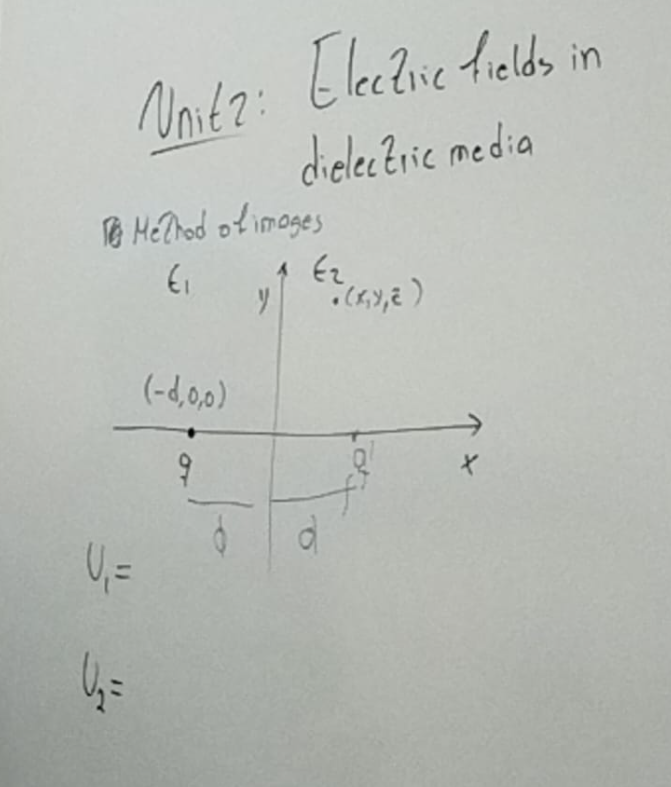
\includegraphics[width=0.7\textwidth]{1.png} % ajusta el ancho según convenga
    \caption{Descripción clara y concisa de la figura.}
    \label{fig:mi_figura} % opcional: para usar con \ref{fig:mi_figura}
\end{figure}

Tenemos $\ldots$

In dielectric 1:

\[   U_{1} = \frac{1}{4\pi \epsilon_{1}} \left[  \frac{q}{r} + \frac{q^{\prime}}{r^{\prime}}  \right] \quad \text{con} \quad r= \sqrt{ (x+d)^{2} + y^{2} + z^{2} } \quad \text{y} \quad r^{\prime} = \sqrt{ (x-d)^{2}+y^{2}+z^{2}  } \]


In dielectric 2 we have:


\[   U_{2} = \frac{ q^{{\prime}{\prime}}  }{4\pi \epsilon_{2}r}     \]


 \begin{figure}[H]
    \centering
    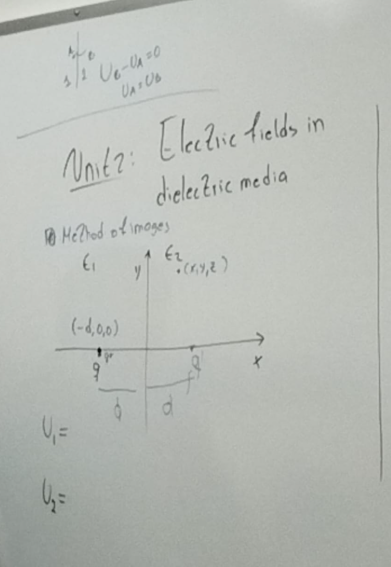
\includegraphics[width=0.7\textwidth]{2.png} % ajusta el ancho según convenga
    \caption{Descripción clara y concisa de la figura.}
    \label{fig:mi_figura} % opcional: para usar con \ref{fig:mi_figura}
\end{figure}



\textbf{Ecuación de Laplace}


\[ \nabla^{2}{U_{1}}=0  \]

\[ \nabla^{2}{U_{2}}=0  \]


\textbf{Remember that:}

\begin{enumerate}
\item $\left. U_{1}\right|_{S} = \left. U_{2}\right|_{S} $
\item $E_{1t} = E_{2t}$
\item $D_{2n}-D_{1n}=\sigma_{S}$
\end{enumerate}

\emph{El campo eléctrico produce la polarización debido al campo eléctrico de la carga}.


\textbf{Actividad:}

\begin{enumerate}
\item[2] [...]\\
\item[3] [...] \\
\item[1] [...]
\end{enumerate}


Tenemos:

\textbf{Remember that:}
\[
\left. U_{1}\right|_{S} = \left. U_{2}\right|_{S},\qquad
E_{1t}=E_{2t},\qquad
D_{2n}-D_{1n}=\sigma_S.
\]

\textcolor{Apple Green}{\textbf{Resolviendo}}

Para el caso \textbf{(2)}, tenemos:

\[   \left. - \frac{ \partial U_{1} }{  \partial y } \right|_{x=0} = \left. - \frac{ \partial U_{2} }{  \partial y } \right|_{x=0}    \]

\begin{equation*}
\begin{split}
&\textbf{Potenciales:}\qquad
U_1=\frac{1}{4\pi\varepsilon_1}\!\left(\frac{q}{r}+\frac{q'}{r'}\right),\qquad
U_2=\frac{1}{4\pi\varepsilon_2}\frac{q''}{r},\\[4pt]
&\text{en } x=0:\; r=r'=:r_S=\sqrt{d^2+y^2+z^2}.
\\[6pt]
&\textbf{Cond. (1) continuidad de }U:\qquad
\left.U_1\right|_{x=0}=\left.U_2\right|_{x=0}
\;\Longrightarrow\;
\frac{q+q'}{\varepsilon_1}=\frac{q''}{\varepsilon_2}.
\\[6pt]
&\textbf{Cond. (2) continuidad de }E_t:\quad
-\partial_y U_1|_{x=0}=-\partial_y U_2|_{x=0},
\ \ \partial_y\!\left(\frac{1}{r}\right)\!=\!\frac{y}{r_S^3}
\\
&\hspace{3.3cm}\Longrightarrow\;
\frac{1}{4\pi}\frac{y}{r_S^3}
\left(\frac{q+q'}{\varepsilon_1}-\frac{q''}{\varepsilon_2}\right)=0
\;\Longrightarrow\;
\frac{q+q'}{\varepsilon_1}=\frac{q''}{\varepsilon_2} \quad(\text{misma que (1)}).
\\[6pt]
&\textbf{Cond. (3) normal de }\mathbf D\ \ (\sigma_S=0):\quad
\varepsilon_1\,\partial_x U_1|_{x=0}=\varepsilon_2\,\partial_x U_2|_{x=0},\\
&\partial_x\!\left(\frac{1}{r}\right)=\frac{x+d}{r^3},\quad
\partial_x\!\left(\frac{1}{r'}\right)=\frac{x-d}{r'^3}
\ \Rightarrow\ 
\partial_x U_1|_{x=0}
=\frac{1}{4\pi\varepsilon_1}\frac{d}{r_S^3}\,(q-q'),\ \ 
\partial_x U_2|_{x=0}
=\frac{1}{4\pi\varepsilon_2}\frac{d}{r_S^3}\,q''\\
&\hspace{3.3cm}\Longrightarrow\;
q''=q-q'.
\\[6pt]
&\textbf{Resolviendo}\ \ 
\begin{cases}
\dfrac{q+q'}{\varepsilon_1}=\dfrac{q''}{\varepsilon_2},\\
q''=q-q',
\end{cases}
\ \Longrightarrow\
\boxed{\,q' = q\,\dfrac{\varepsilon_1-\varepsilon_2}{\varepsilon_1+\varepsilon_2}\,},\qquad
\boxed{\,q''= q\,\dfrac{2\varepsilon_2}{\varepsilon_1+\varepsilon_2}\,}.
\end{split}
\end{equation*}


\textcolor{Cinnabar}{\textbf{Solución adecuada}}

\[ - \left( -\frac{1}{2} \right) \frac{  1}{4\pi \epsilon_{1}} \frac{ 2( q+q^{\prime} )y }{( d^{2} + y^{2} + z^{2})^{\frac{3}{2}}} = - \left(  -\frac{1}{2}  \right) \frac{1 }{4\pi\epsilon_{2}} \frac{ 2 q^{{\prime}{\prime}} y}{ ( d^{2} + y^{2} + z^{2} )^{ \frac{3}{2}} }   \]


De acá se tiene:


\[  \frac{  q+q^{\prime} }{ \epsilon_{1} } = \frac{ q^{ {\prime}{\prime}} }{\epsilon_{2}}  \]


Ahora necesitamos aplicar la condición \textbf{(3)}, tenemos: 


\textcolor{Cinnabar}{\textbf{Solución adecuada}}

% --- Condición (2): continuidad de E_t (ya dada por ti) ---
\[
- \left( -\frac{1}{2} \right) \frac{1}{4\pi \epsilon_{1}}
\frac{ 2( q+q^{\prime} )\,y }{( d^{2} + y^{2} + z^{2})^{3/2}}
=
- \left( -\frac{1}{2} \right) \frac{1}{4\pi\epsilon_{2}}
\frac{ 2 q^{\prime\prime}\, y}{ ( d^{2} + y^{2} + z^{2} )^{3/2} }
\]

\[
\Rightarrow\qquad
\boxed{\;\frac{  q+q^{\prime} }{ \epsilon_{1} } = \frac{ q^{ \prime\prime } }{\epsilon_{2}}\;}
\]

% --- Condición (3): salto de D_n (con \sigma_S = 0) ---
\textbf{Ahora, condición (3) (componente normal):}

\[\quad
\epsilon_1 \left.\frac{\partial U_1}{\partial x}\right|_{x=0}
- \epsilon_2 \left.\frac{\partial U_2}{\partial x}\right|_{x=0}
= \sigma_S \quad (\text{aquí tomamos } \sigma_S=0).
\]

\[
U_1=\frac{1}{4\pi\epsilon_1}\!\left(\frac{q}{r}+\frac{q'}{r'}\right),
\qquad
U_2=\frac{1}{4\pi\epsilon_2}\frac{q''}{r},
\quad
\begin{cases}
r=\sqrt{(x+d)^2+y^2+z^2},\\
r'=\sqrt{(x-d)^2+y^2+z^2}.
\end{cases}
\]

\[
\frac{\partial}{\partial x}\!\left(\frac{1}{r}\right)=\frac{x+d}{r^3},
\qquad
\frac{\partial}{\partial x}\!\left(\frac{1}{r'}\right)=\frac{x-d}{r'^3}.
\]

\[
\text{En }x=0:\quad r=r'=:r_S=\sqrt{d^2+y^2+z^2},\ 
\left.\frac{\partial}{\partial x}\!\frac{1}{r}\right|_{0}=\frac{d}{r_S^3},\ 
\left.\frac{\partial}{\partial x}\!\frac{1}{r'}\right|_{0}=-\frac{d}{r_S^3}.
\]

\[
\Rightarrow\ 
\left.\frac{\partial U_1}{\partial x}\right|_{0}
=\frac{1}{4\pi\epsilon_1}\frac{d}{r_S^3}(q-q'),
\qquad
\left.\frac{\partial U_2}{\partial x}\right|_{0}
=\frac{1}{4\pi\epsilon_2}\frac{d}{r_S^3}\,q''.
\]

\[
\epsilon_1 \left.\frac{\partial U_1}{\partial x}\right|_{0}
- \epsilon_2 \left.\frac{\partial U_2}{\partial x}\right|_{0}=0
\ \Longrightarrow\
\frac{d}{4\pi r_S^3}\,(q-q' - q'')=0
\ \Longrightarrow\
\boxed{\;q''=q-q'\;}
\]

% --- Resolviendo el sistema de 2 ecuaciones ---
\[
\begin{cases}
\dfrac{q+q'}{\epsilon_1}=\dfrac{q''}{\epsilon_2},\\[6pt]
q''=q-q',
\end{cases}
\quad\Longrightarrow\quad
\boxed{\,q' = q\,\dfrac{\epsilon_1-\epsilon_2}{\epsilon_1+\epsilon_2}\,},
\qquad
\boxed{\,q'' = q\,\dfrac{2\epsilon_2}{\epsilon_1+\epsilon_2}\,}.
\]

\textcolor{Cerulean}{\textbf{Solcuión correcta (3)}} $\ldots$ tenemos:

La condicion 1 es redudnate con la \textbf{condición 2}, para cualquier $y$ y $z$ se satisface la ecuación

\begin{equation}
\begin{split} 
 \left. - \epsilon_{1} \frac{  \partial U_{1} }{\partial x} \right|_{x=0}   &= \left. - \epsilon_{2} \frac{  \partial U_{2} }{\partial x} \right|_{x=0}\\
\frac{-\epsilon_{1} \left( -\frac{1}{2} \right)}{4\pi\epsilon_{1}}  \frac{  (q-q^{\prime}) (2d) }{ (d^{2} + y^{2} +z^{2})^{\frac{3}{2}} }  &= \frac{\epsilon_{2} \left( -\frac{1}{2} \right)}{4\pi\epsilon_{2}}  \frac{ 2(-d)  (q^{{\prime}{\prime}}) }{ (d^{2} + y^{2} +z^{2})^{\frac{3}{2}} }
\end{split}
\end{equation}

\text{para la parte derecha de esta ecuación, signo menos de $\epsilon_{2}$ se va por ser normal}


\[ -\epsilon_{2} \]

Tenemos: 


 \begin{figure}[H]
    \centering
    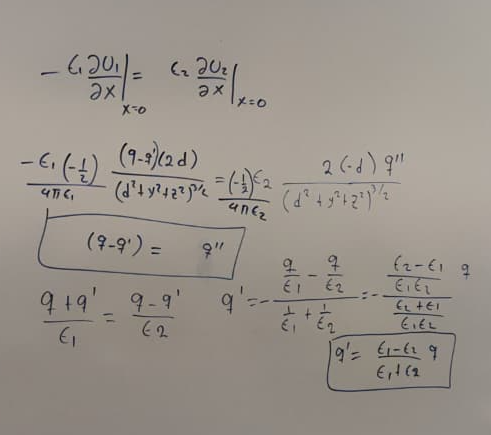
\includegraphics[width=0.7\textwidth]{3.png} % ajusta el ancho según convenga
    \caption{Descripción clara y concisa de la figura.}
    \label{fig:mi_figura} % opcional: para usar con \ref{fig:mi_figura}
\end{figure}

 \begin{figure}[H]
    \centering
    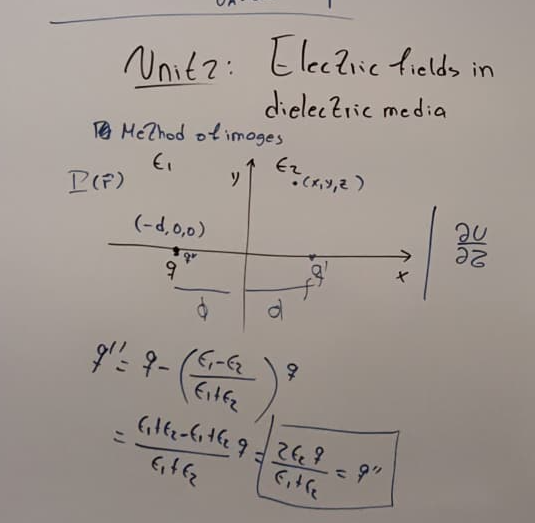
\includegraphics[width=0.7\textwidth]{4.png} % ajusta el ancho según convenga
    \caption{Descripción clara y concisa de la figura.}
    \label{fig:mi_figura} % opcional: para usar con \ref{fig:mi_figura}
\end{figure}


Todo se reduce a un problema algebraico. 

\textbf{Nueva sección}

Tenemos un dieléctrico homogéneo. Definimos la \emph{polarización} como el momento dipolar por unidad de volumen:
\[
\mathbf{P}=\lim_{\Delta V\to 0}\frac{\Delta \mathbf{p}}{\Delta V}.
\]

Las \emph{cargas ligadas} (de polarización) se obtienen de:
\[
\rho_b=-\nabla\cdot\mathbf{P},\qquad \sigma_b=\mathbf{P}\cdot\hat{\mathbf n}.
\]

Además, el campo de desplazamiento verifica
\[
\mathbf{D}=\varepsilon_0\mathbf{E}+\mathbf{P},\qquad \nabla\cdot\mathbf{D}=\rho_{\text{libre}}.
\]

\textbf{Conexión molecular y constitutiva}

Para un dieléctrico lineal e isótropo:
\[
\mathbf{P}=\varepsilon_0\chi_e\,\mathbf{E},\qquad 
\mathbf{P}=N\,\alpha\,\mathbf{E}_{\text{local}},\qquad 
\frac{\varepsilon_r-1}{\varepsilon_r+2}=\frac{N\alpha}{3\varepsilon_0}.
\]

\textbf{Campo local en una cavidad esférica}

El campo que “ve” una molécula se descompone como
\[
\mathbf{E}_{\text{local}}=\mathbf{E}_{\text{macro}}+\frac{\mathbf{P}}{3\varepsilon_0}+\mathbf{E}^{\,\prime},
\]
donde $\mathbf{E}_{\text{macro}}$ es el campo promedio, $\mathbf{P}/(3\varepsilon_0)$ es el
\emph{campo de Lorentz} (debido a la carga ligada en la superficie de una cavidad esférica),
y $\mathbf{E}^{\,\prime}$ es el campo de los dipolos cercanos (contribución microscópica).


Donde $E_{d}$ campo eléctrico de polarización. $E^{\prime}$ campo eléctrico nativo de las moléculas	

Carga de polarización superficial es la que importa y existen dos tipos de esa carga (\textbf{Se verá la siguiente clase}).



\textbf{Hasta acá finaliza la clase $\ldots$ continuamos la siguiente clase}




% ====== Problema de Laplace con condiciones de frontera mixtas
% ====== en dos subdominios con interfaz






\end{document}